\documentclass[../sparc.tex]{subfiles}
\graphicspath{{\subfix{../images/}}}
\begin{document}

\section{Sound}
\index{Music!Sound frequency}
\newglossaryentry{Hz}{name=Hz, description={Hertz}}
\newglossaryentry{kHz}{name=kHz, description={Kilohertz ($10^3$ Hz)}}
\newglossaryentry{MHz}{name=MHz, description={Megahertz ($10^6$ Hz)}}
\newglossaryentry{GHz}{name=GHz, description={Gigahertz ($10^9$ Hz)}}

As it is commonly known, \emph{sound} is a mechanical disturbance from a state
of equilibrium that propagates through some medium (such as the air) in a form
of an acoustic wave. \cite{britannica:sound}

As a wave it one of the main parameters of the sound is its \emph{frequency}.

Frequencies are measured in \emph{Hertz} (\gls{Hz}), and one Hertz (1 Hz) means
one oscillation per second.  10 oscillations per seconds gives us 10 Hz, 100
oscillations per second gives us 100 Hz and so on.  When we are talking about
1000 Hz or more, it is more convenient to use standard multiples of a Hertz:
``Kilo-'' (\gls{kHz}), ``Mega-'' (\gls{MHz}) and ``Giga-'' (\gls{GHz}).

Some of the common multiples of a Hertz are shown in the table below.

\begin{table}[h]
  \centering
  \begin{tabular}{p{3cm}|p{4cm}|p{3.5cm}}
    Measurement unit & Relation to Hertz & Examples \\
    \hline \hline
    Hertz (Hz)
    & $ 1 \mbox{Hz} $ or $ 10^0 \mbox{Hz} $
    & $ 100 * 10^0 \mbox{Hz} = 100 \mbox{Hz} $ \\
    \hline
    Kilohertz (kHz)
    & $ 1000 \mbox{Hz} $ or $ 10^3 \mbox{Hz} $
    & $ 100 * 10^3 \mbox{Hz} = 100 \mbox{kHz} $ \\
    \hline
    Megahertz (MHz)
    & $ 1000000 \mbox{Hz} $ или $ 10^6 \mbox{Hz} $
    & $ 100 * 10^6 \mbox{Hz} = 100 \mbox{MHz} $ \\
    \hline
    Gigahertz (GHz)
    & $ 1000000000 \mbox{Hz} $ или $ 10^9 \mbox{Hz} $
    & $ 100 * 10^9 \mbox{Hz} = 100 \mbox{GHz} $ \\
  \end{tabular}
  \caption{Some units of the frequency measurement.}
  \label{table:sound-hertz-scale}
\end{table}

Thus we need to know the sound frequency to an acoustic wave with proper wave
length to make that sound.  And vice versa, when we know the wave length, we can
calculate the sound frequency from it.  This can be visualized as is shown on
fig. \ref{fig:sound-fig-1}.

\begin{figure}[h]
  \centering
  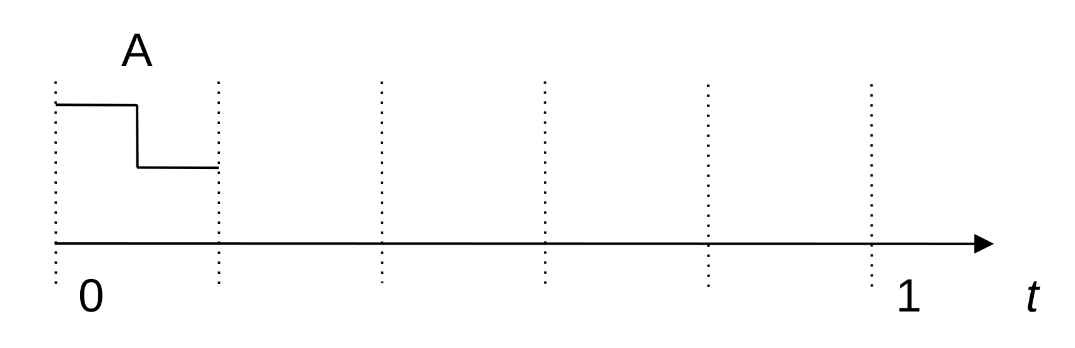
\includegraphics[width=10cm]{sound-fig-1}
  \caption{A visual representation of an acoustic wave with the frequency of 5
    Hz.}
  \label{fig:sound-fig-1}
\end{figure}

If we know that an oscillation can be fit 5 times on 1 second we say that the
frequency of such wave has the frequency of 5 Hz.  If we want to calculate the
period duration, we can divide 1 second (specified in microseconds) by the
frequency:

\begin{equation}
  \frac{1000000 \mu\mbox{s}}{5 \mbox{Hz}} = 200000 \mu\mbox{s}
\end{equation}

Which means that the wave length is 200000 $\mu\mbox{s}$, or $ 200 * 10^3
\mbox{ms}$.  If we know the wavelength and want to know the frequency we can
divide 1 second (in microseconds) by the wavelength and by that we will get the
frequency (in Hertz).  That's easy.

The method of sound generation is similar to \gls{PWM}.  The main difference is
that now we must change the wavelength, keeping the duty cycle constant.

\end{document}
